\section{Simulation Results}
\label{sec:results}

\begin{table*}[t]
\centering
\caption{Overall comparison on the BEAR OfficeSmall-Hot\_Dry task. Energy is the average HVAC energy per episode. Violations denote the average thermal comfort violations. Reward is the final test reward averaged over the last five checkpoints. For the action smoothness metric, lower mean absolute action change indicates smoother control.}
\label{tab:overall_results}
\setlength{\tabcolsep}{6pt}
\renewcommand{\arraystretch}{1.12}
\begin{tabular}{lcccc}
\hline
Method & Energy (kWh) $\downarrow$ & Violations $\downarrow$ & Test Reward $\uparrow$ & Mean $|\Delta a|$ $\downarrow$ \\
\hline
Guided-DiffFNO & 877.3 & \textbf{0.605} & \textbf{-0.557} & \textbf{0.0244} \\
DiffFNO w/o Guidance & 895.7 & 1.380 & -1.037 & 0.0471 \\
DiffFNO w/o Residual \& Guidance & \textbf{861.5} & 1.002 & -0.794 & 0.0344 \\
DiffFNO w/o Residual & 866.9 & 0.707 & -0.615 & \textbf{0.0244} \\
Diffusion Policy (MLP backbone) & 1106.2 & 1.449 & -1.147 & 0.0964 \\
MPC & 1004.9 & 1.780 & -1.325 & -- \\
SAC & 5897.0 & 5.680 & -5.560 & 0.3970 \\
SAC+MPC & 1934.6 & 3.462 & -2.640 & 0.1656 \\
\hline
\end{tabular}
\end{table*}

\begin{figure}[t]
\centering
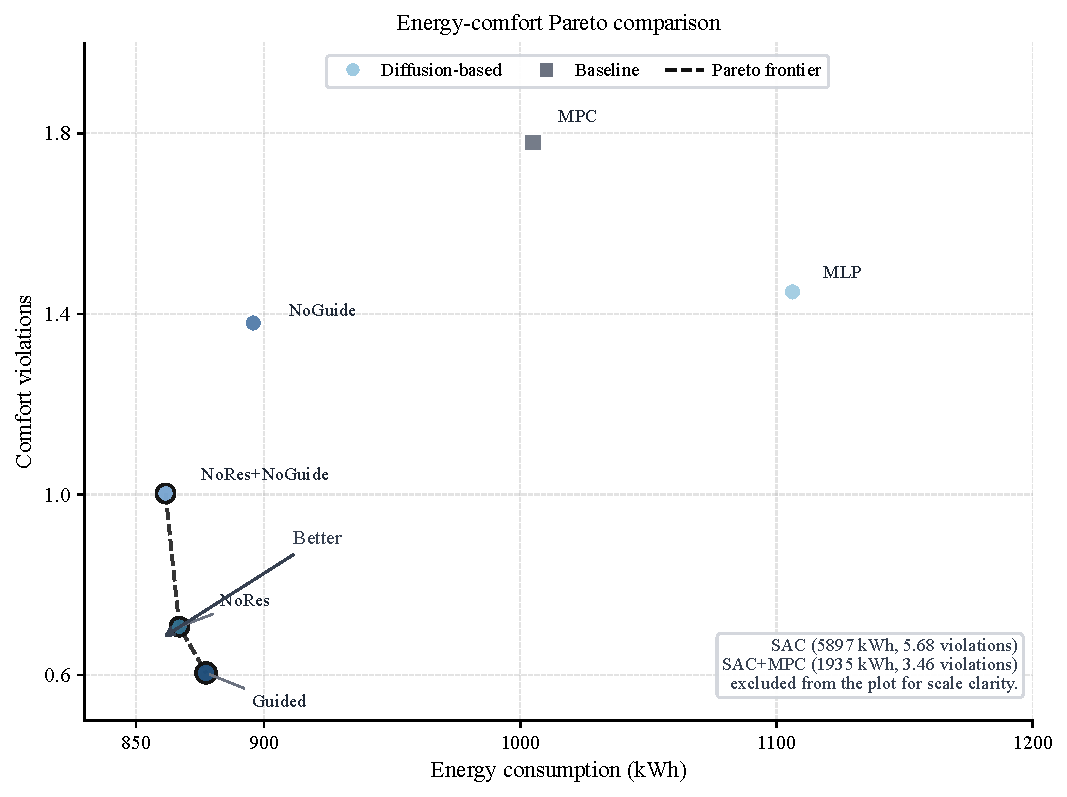
\includegraphics[width=\linewidth]{paperfigure/compare_energy_violations.pdf}
\caption{Energy--comfort Pareto comparison in the practically relevant performance region. Each point summarizes the average HVAC energy consumption and average comfort violations over the last five evaluation checkpoints. Lower-left is better. The dashed line connects the non-dominated methods. For scale clarity, the highly suboptimal SAC and SAC+MPC baselines are omitted from the scatter plot but still reported in Table~\ref{tab:overall_results}.}
\label{fig:energy_violations}
\end{figure}

\subsection{Overall Energy--Comfort Trade-off}

Table~\ref{tab:overall_results} and Fig.~\ref{fig:energy_violations} summarize the main quantitative results. The Pareto view is particularly informative here because the HVAC task is intrinsically bi-objective: a controller is only practically meaningful if it reduces energy use while simultaneously maintaining comfort compliance. Under this view, the non-dominated frontier in Fig.~\ref{fig:energy_violations} is formed by three diffusion-based variants only, namely DiffFNO w/o Residual \& Guidance, DiffFNO w/o Residual, and Guided-DiffFNO. All other displayed methods are dominated in the energy--comfort plane. In particular, DiffFNO w/o Guidance is shown in the scatter plot as a dominated reference point, but it is not connected by the dashed Pareto line because DiffFNO w/o Residual \& Guidance improves both objectives simultaneously, reducing energy from $895.7$~kWh to $861.5$~kWh and violations from $1.380$ to $1.002$.

Among these frontier methods, Guided-DiffFNO occupies the most desirable safety-oriented end of the trade-off curve. It achieves the lowest comfort violation score of $0.605$ and the highest final test reward of $-0.557$, while keeping the average HVAC energy at $877.3$~kWh. By contrast, DiffFNO w/o Residual \& Guidance attains the lowest raw energy value ($861.5$~kWh), but does so at substantially worse comfort compliance ($1.002$ violations) and lower final reward ($-0.794$). This distinction is important: from the perspective of building control, minimizing HVAC power alone is not a sufficient objective, because a useful controller must optimize energy and thermal safety jointly rather than overfitting to one side of the trade-off. Guided-DiffFNO therefore provides the best balanced solution among all compared methods.

The contribution of critic-guided reverse sampling is directly visible in this comparison. Relative to the unguided DiffFNO variant, Guided-DiffFNO reduces energy consumption from $895.7$~kWh to $877.3$~kWh and cuts comfort violations from $1.380$ to $0.605$, corresponding to a $2.1\%$ reduction in energy and a $56.2\%$ reduction in violations. The final test reward also improves from $-1.037$ to $-0.557$. Notably, the unguided model does not lie on the Pareto frontier because it is simultaneously outperformed by DiffFNO w/o Residual \& Guidance in both energy and comfort. This observation indicates that value-guided refinement is not merely a cosmetic adjustment to the final sampled action, but materially changes the denoising trajectory toward higher-value and safer control decisions.

The comparison with non-spectral and conventional baselines is even more pronounced. Relative to the MLP-based diffusion policy, Guided-DiffFNO reduces energy by $20.7\%$ and comfort violations by $58.3\%$. Relative to MPC, the proposed method lowers energy by $12.7\%$ and violations by $66.0\%$. The excluded SAC and SAC+MPC baselines, although omitted from Fig.~\ref{fig:energy_violations} for scale clarity, remain important as negative references in Table~\ref{tab:overall_results}: SAC consumes $5897.0$~kWh with $5.680$ violations, while SAC+MPC still consumes $1934.6$~kWh with $3.462$ violations. These results indicate that standard unimodal actor policies, even when aided by expert regularization, remain poorly matched to the strongly coupled multi-zone HVAC control problem.

\begin{figure}[t]
\centering
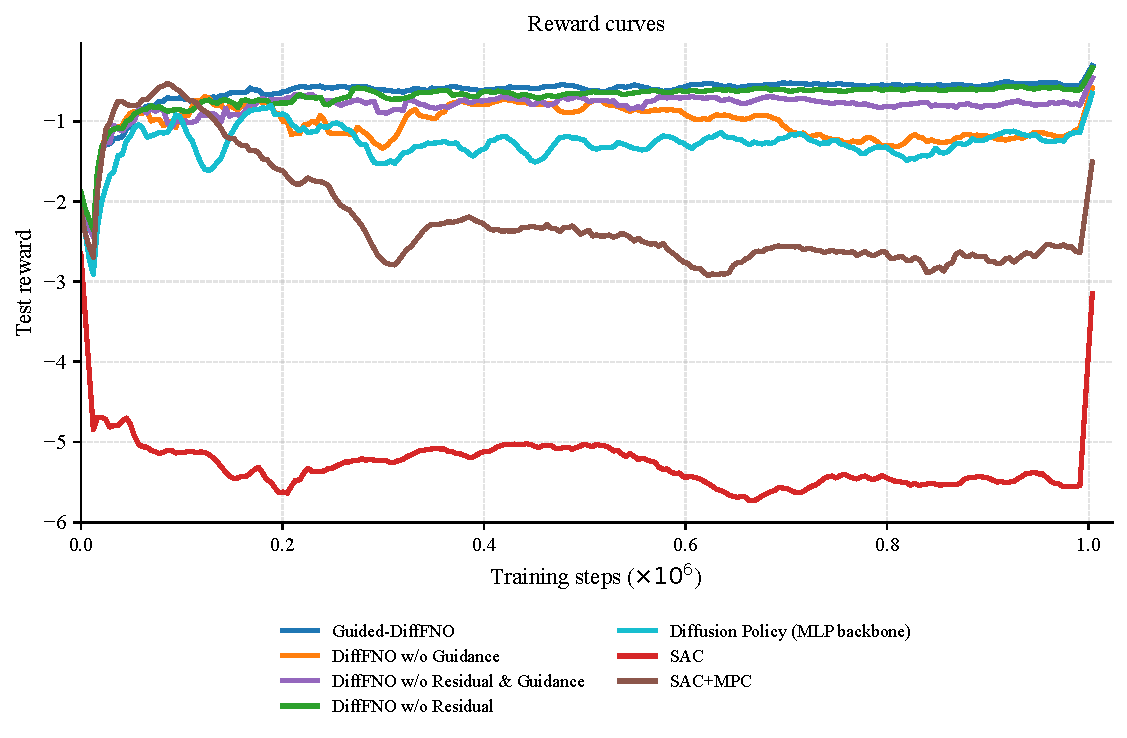
\includegraphics[width=\linewidth]{paperfigure/compare_reward_curves.pdf}
\caption{Test reward curves during training. Higher is better.}
\label{fig:reward_curves}
\end{figure}

\subsection{Training Dynamics and Optimization Stability}

The training curves in Fig.~\ref{fig:reward_curves} reveal a clear difference in optimization stability. Guided-DiffFNO is the only method that maintains a strong reward level throughout most of training and finishes with the best final performance. Its reward already improves to approximately $-0.578$ at $2.5\times 10^5$ environment steps, remains around the $-0.53$ to $-0.60$ range over the second half of training, and reaches its best checkpoint value of $-0.453$ near $7.99\times 10^5$ steps.

By contrast, the unguided DiffFNO variant exhibits much larger oscillations and finishes significantly worse than the guided model. The MLP-based diffusion policy also fails to maintain stable improvement and gradually degrades as training proceeds. SAC+MPC shows a strong initial reward due to expert regularization, but this advantage quickly collapses; after an early best value of $-0.391$ around $7.37\times 10^4$ steps, its performance steadily deteriorates and ends at a much lower level than Guided-DiffFNO. This behavior suggests that imitation alone is insufficient to stabilize long-horizon policy improvement unless the policy class itself can preserve a structured action prior. Pure SAC is unstable from the beginning and never enters the reward regime reached by the diffusion-based methods.

These results indicate that the combination of diffusion-based action modeling, FNO-induced structural bias, and inference-time critic refinement leads to a better optimization landscape than either conventional actor-critic training or unguided denoising alone.

\begin{figure}[t]
\centering
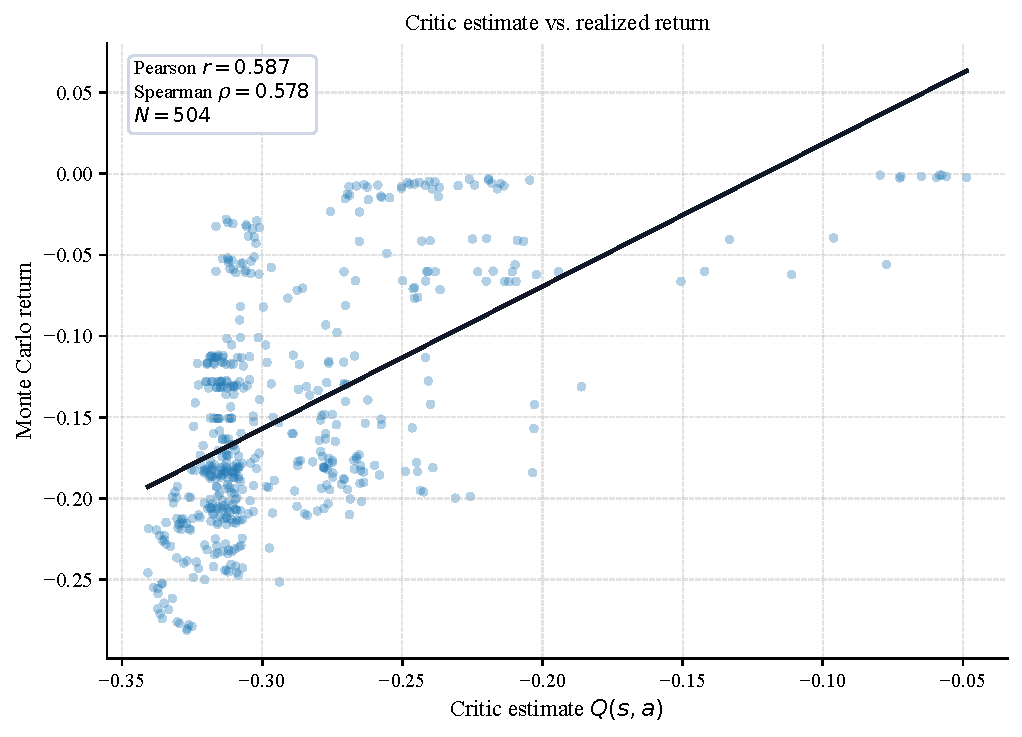
\includegraphics[width=0.88\linewidth]{paperfigure/critic_q_mc_return.pdf}
\caption{Relation between critic-estimated $Q(s,a)$ and Monte Carlo return for Guided-DiffFNO, computed from logged evaluation transitions.}
\label{fig:q_mc_return}
\end{figure}

\subsection{Mechanism Validation of Critic Guidance}

Because the proposed guidance term is derived from the critic gradient, it is important to verify that the critic provides a meaningful value signal rather than an arbitrary directional perturbation. Figure~\ref{fig:q_mc_return} addresses this point by plotting the critic-estimated $Q(s,a)$ against the corresponding Monte Carlo return on logged evaluation samples. The two quantities exhibit a clear positive association, with Pearson correlation $r=0.587$ and Spearman rank correlation $\rho=0.578$ over $N=504$ state--action pairs collected from the logged evaluation trajectories.

This result should not be interpreted as perfect critic calibration; such a claim would be too strong for an off-policy continuous-control setting. However, it does show that the learned critic preserves a useful ranking relationship between actions with lower and higher long-term return. From the perspective of guided diffusion, this is the relevant property: the critic does not need to provide an exact return estimator at every point in action space, but it does need to induce gradients that preferentially move the denoising process toward higher-value regions. The significant improvement of Guided-DiffFNO over unguided DiffFNO in both reward and comfort violations, together with the positive $Q$--return relation in Fig.~\ref{fig:q_mc_return}, therefore supports the claim that critic guidance is functioning as an effective inference-time refinement mechanism.

\begin{figure}[t]
\centering
\begin{minipage}[t]{0.48\linewidth}
\centering
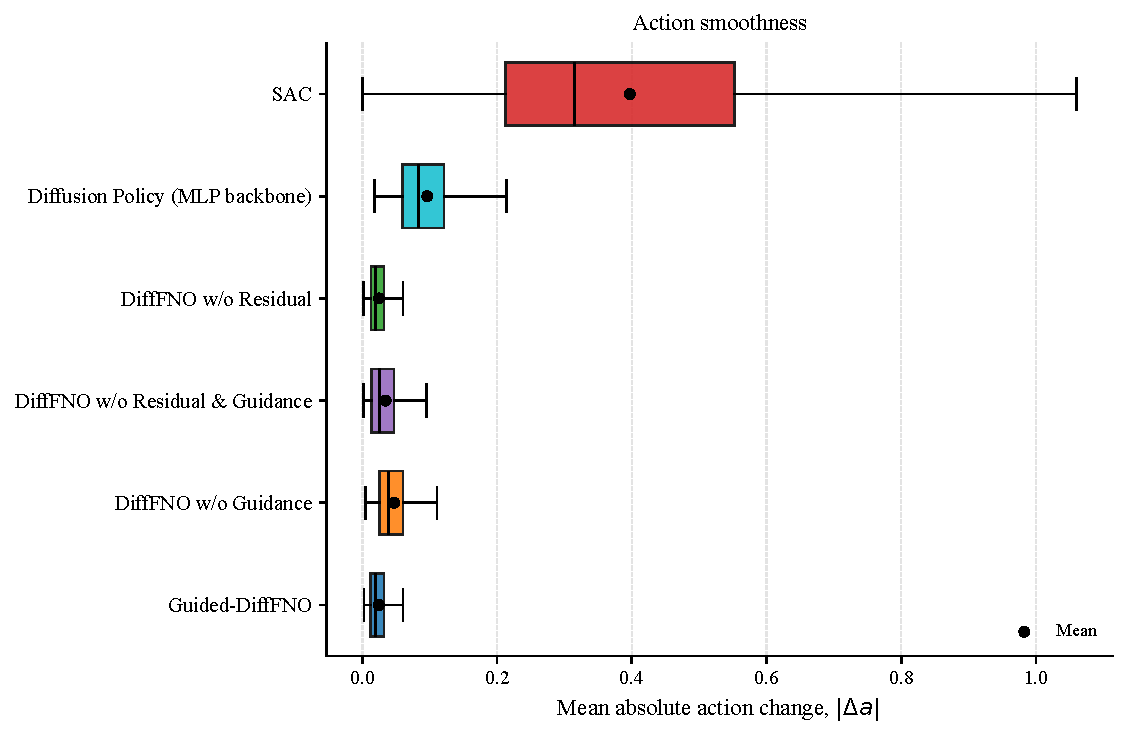
\includegraphics[width=\linewidth]{paperfigure/compare_action_smoothness.pdf}
\end{minipage}
\hfill
\begin{minipage}[t]{0.48\linewidth}
\centering
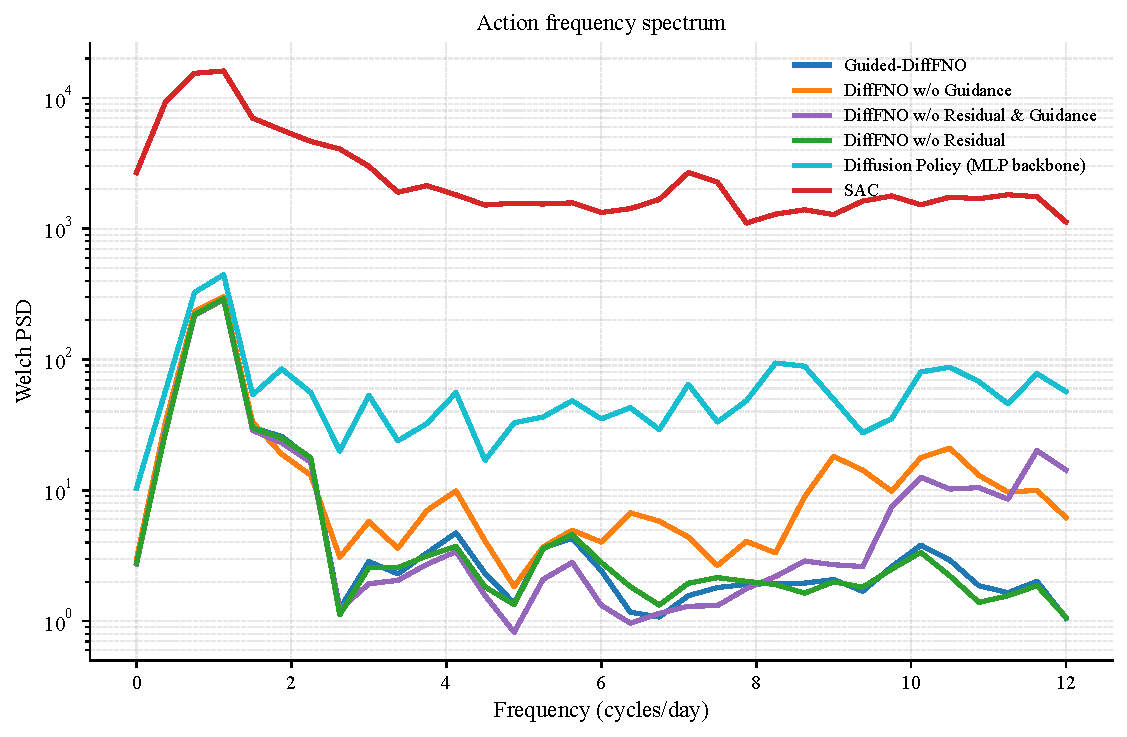
\includegraphics[width=\linewidth]{paperfigure/action_psd_compare.pdf}
\end{minipage}
\caption{Action-quality analysis. Left: distribution of mean absolute action changes. Right: Welch power spectral density (PSD) of generated actions. For each method, the PSD is computed from the logged evaluation trajectories using a sampling frequency of $f_s=1/3600$ Hz (one control step per hour), Welch window length $n_{\mathrm{seg}}=64$, and overlap $32$. Let $S_j(f_m)$ denote the discrete Welch spectrum of control dimension $j$ at frequency bin $f_m$. The plotted spectrum is the cross-zone average $S(f_m)=\frac{1}{6}\sum_{j=1}^{6}S_j(f_m)$. All high-frequency ratios reported below are computed from these discrete bins by summing the spectral mass above the prescribed cutoff.}
\label{fig:action_quality}
\end{figure}

\begin{figure}[t]
\centering
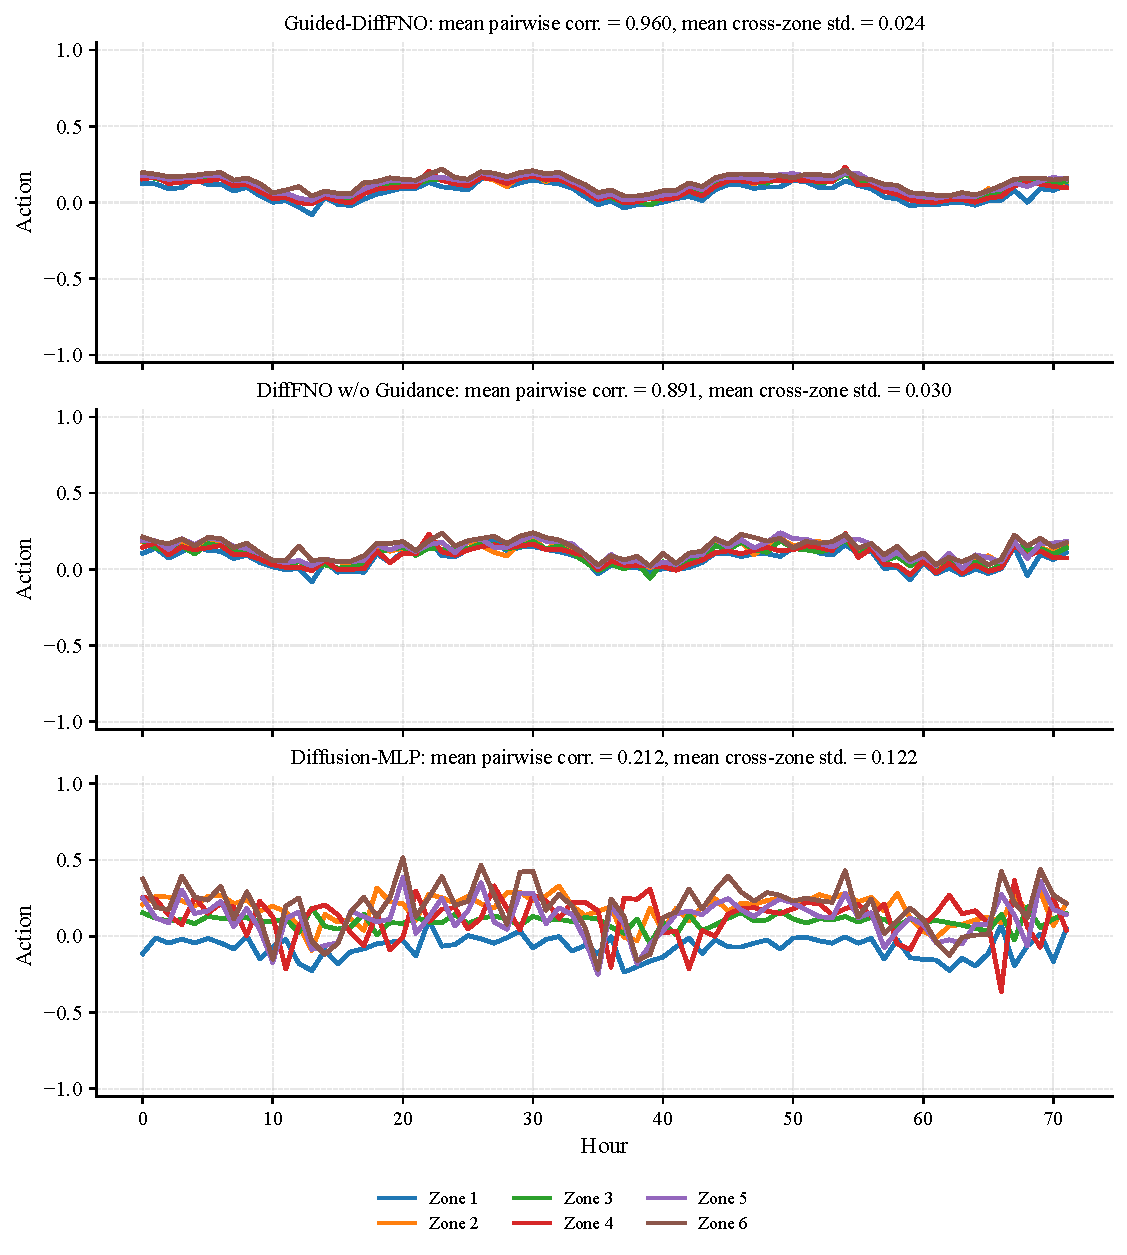
\includegraphics[width=\linewidth]{paperfigure/multizone_action_coordination.pdf}
\caption{Multi-zone action coordination over a representative 72-hour window for Guided-DiffFNO, DiffFNO w/o Guidance, and Diffusion-MLP. Guided-DiffFNO exhibits the strongest inter-zone consistency while preserving meaningful zone-to-zone variation; the unguided DiffFNO baseline remains coordinated but weaker, and the MLP-based diffusion policy produces visibly more scattered and less coordinated control signals.}
\label{fig:multizone_coordination}
\end{figure}

\begin{figure}[t]
\centering
\begin{minipage}[t]{0.48\linewidth}
\centering
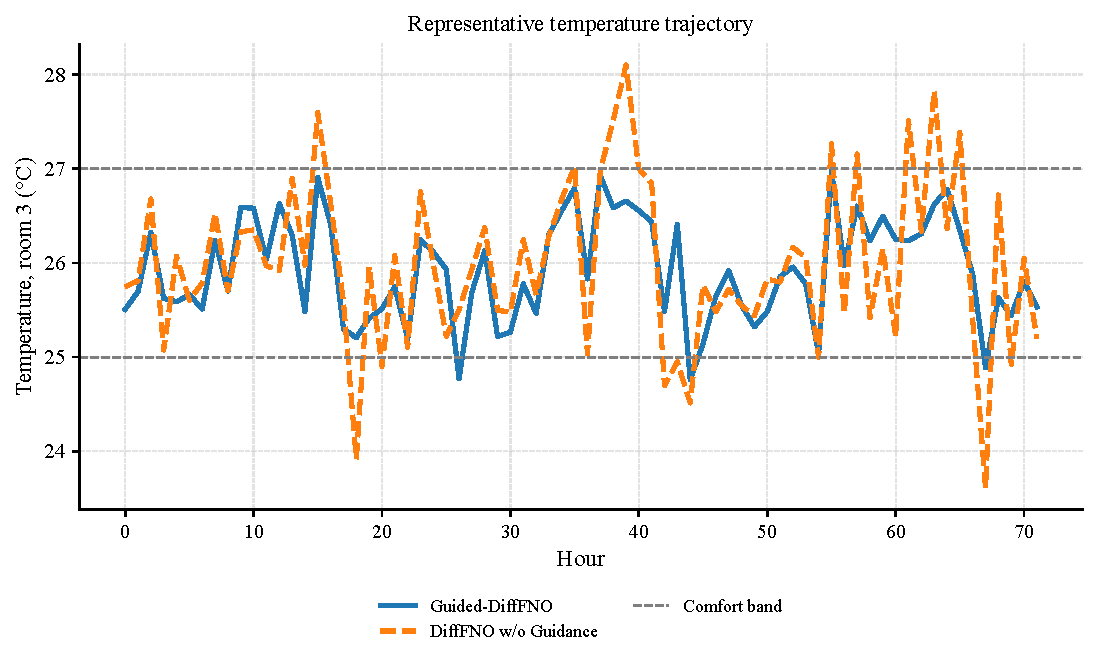
\includegraphics[width=\linewidth]{paperfigure/temperature_trajectories_paper.pdf}
\end{minipage}
\hfill
\begin{minipage}[t]{0.48\linewidth}
\centering
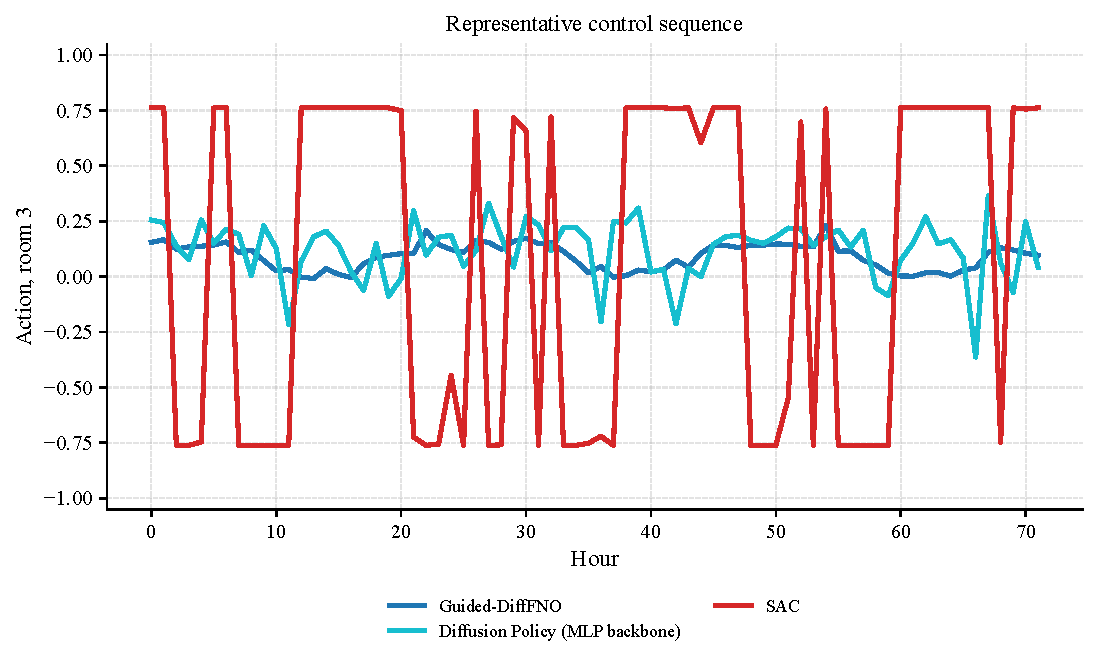
\includegraphics[width=\linewidth]{paperfigure/control_sequence_paper.pdf}
\end{minipage}
\caption{Representative trajectories for a selected room. Left: temperature evolution under Guided-DiffFNO and unguided DiffFNO. Right: control sequences generated by Guided-DiffFNO, Diffusion-MLP, and SAC.}
\label{fig:traj_control}
\end{figure}

\subsection{Action Quality and Physical Consistency}

Beyond scalar reward and energy metrics, the proposed method also produces substantially smoother and more physically plausible control trajectories. As shown in Fig.~\ref{fig:action_quality}, Guided-DiffFNO achieves the lowest action-variation level among the evaluated learned controllers, with mean absolute action change $0.0244$. This is nearly identical to the no-residual guided variant, but much lower than unguided DiffFNO ($0.0471$), Diffusion-MLP ($0.0964$), SAC+MPC ($0.1656$), and SAC ($0.3970$). Relative to Diffusion-MLP, the full model reduces average action variation by $74.7\%$, which confirms that the FNO backbone is effective in suppressing control chatter in the joint action space.

Figure~\ref{fig:multizone_coordination} provides a direct visualization of the cross-zone coordination claim that motivates the FNO backbone. This figure is particularly important because the single-room trajectories in Fig.~\ref{fig:traj_control} alone could otherwise be interpreted as a representative but potentially cherry-picked local example. Over the same 72-hour window, the six zone actions generated by Guided-DiffFNO evolve in a highly synchronized manner, with mean pairwise inter-zone correlation $0.960$ and mean cross-zone standard deviation $0.024$. The high correlation should not be interpreted as the policy collapsing all zone commands to an identical scalar profile. Rather, it indicates that different zones respond coherently to the same global disturbances and operating rhythm, such as weather and daily load cycles, while still retaining nonzero zone-specific variation. This remaining differentiation is reflected by the nonzero cross-zone standard deviation, which stays at $0.024$ for Guided-DiffFNO and is substantially smaller than the much less structured $0.122$ observed for the MLP-based diffusion policy.

Importantly, adding DiffFNO w/o Guidance to the same visualization clarifies that the structural benefit is not created solely by critic guidance. The unguided DiffFNO baseline already exhibits relatively strong inter-zone coordination, with mean pairwise correlation $0.891$ and mean cross-zone standard deviation $0.030$, placing it clearly between Guided-DiffFNO and Diffusion-MLP. This three-way comparison therefore supports a more precise interpretation of the method components: the FNO backbone is the main source of coordinated multi-zone action structure, whereas critic guidance further sharpens that structure and improves the final energy--comfort trade-off.

In contrast, the MLP-based diffusion policy exhibits much weaker agreement across zones, with mean pairwise correlation only $0.212$. This comparison directly supports the structural hypothesis of the paper: the FNO backbone is not merely smoother in a generic sense, but specifically better at producing joint control vectors that remain globally coherent across coupled thermal zones without degenerating to identical outputs.

The frequency-domain analysis further supports this conclusion. Let $\{f_m\}_{m=1}^{M}$ denote the discrete Welch frequency bins and let $S(f_m)$ denote the averaged spectrum shown in Fig.~\ref{fig:action_quality}. Because the stored PSD is discrete rather than continuous, the reported high-frequency ratio is computed by the same discrete summation used in the figure post-processing:
\begin{equation}
\rho_{\mathrm{HF}}=\frac{\sum_{m:\,f_m>2\ \mathrm{cpd}} S(f_m)}{\sum_{m=1}^{M} S(f_m)},
\label{eq:hf_ratio}
\end{equation}
where ``cpd'' denotes cycles per day. Under the hourly control interval, the cutoff of $2$ cycles/day corresponds to oscillations faster than one cycle every 12 hours. We use this threshold as an explicit analysis convention in this paper to distinguish daily or slower actuation structure from visibly faster control chatter; it should therefore be interpreted as an operational cutoff for comparing policies, rather than as a universal physical constant. With this discrete definition, Guided-DiffFNO allocates $11.4\%$ of its spectral mass to the high-frequency region, compared with $25.8\%$ for unguided DiffFNO and $57.8\%$ for Diffusion-MLP. All learned methods still exhibit a dominant spectral peak around $1.125$ cycles/day, which is consistent with the daily rhythm of building thermal disturbances. Therefore, the proposed approach does not remove the meaningful low-frequency control structure associated with building operation; instead, it selectively suppresses spurious high-frequency oscillations that are unlikely to be physically desirable.

The time-domain trajectories in Fig.~\ref{fig:traj_control} provide a concrete room-level illustration of the same behavior. Over the representative evaluation window, the selected room under Guided-DiffFNO leaves the comfort band only $3$ times out of $72$ control steps, whereas the unguided DiffFNO leaves the band $17$ times and the Diffusion-MLP controller produces far larger excursions. In the same window, the room-wise action sequence generated by Guided-DiffFNO has mean step-to-step variation $0.0259$, compared with $0.0415$ for unguided DiffFNO, $0.1384$ for Diffusion-MLP, and $0.4387$ for SAC. SAC also exhibits extreme temperature excursions, with the selected-room state ranging from $-9.10^\circ$C to $43.15^\circ$C. These values should be interpreted as raw simulator state outputs under destabilizing control inputs after the closed-loop system has left the normal operating regime, rather than as realistic occupied-zone temperatures in a physically meaningful HVAC trajectory. In other words, they are evidence of severe control-induced instability in the simulator response, which is precisely why we use them as a symptom of poor physical consistency.

Taken together, these results support the central design claim of this paper: for multi-zone HVAC control, a good policy should not only optimize aggregate reward, but should also generate coordinated joint actions whose temporal and spectral characteristics remain compatible with the physics of coupled building dynamics.

\begin{figure}[t]
\centering
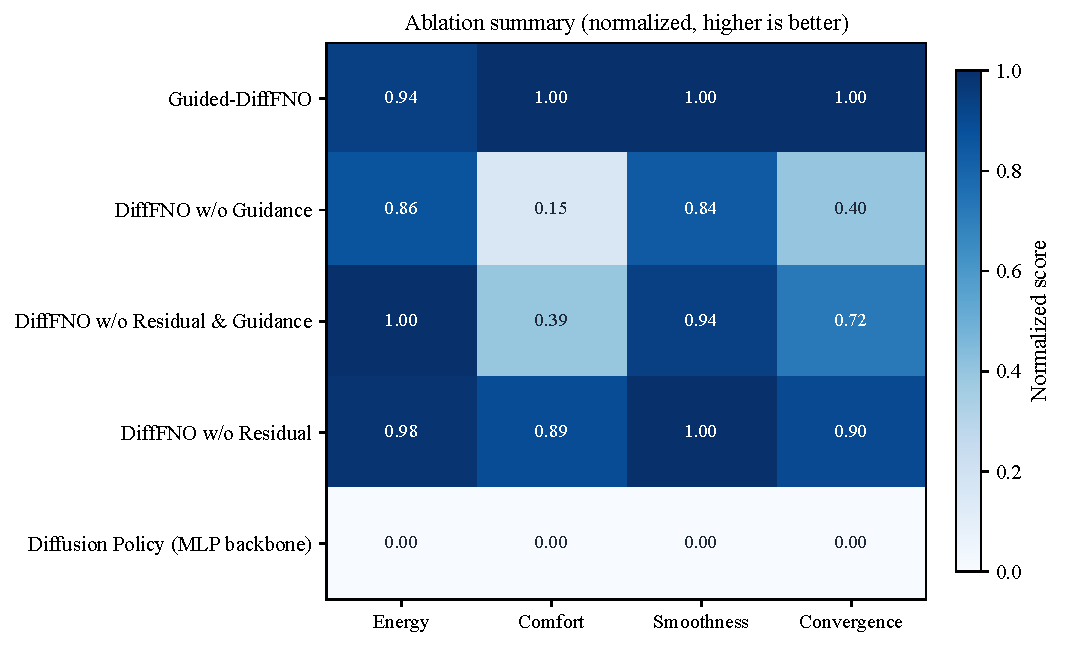
\includegraphics[width=\linewidth]{paperfigure/ablation_summary_heatmap.pdf}
\caption{Normalized ablation summary across energy, comfort, smoothness, and convergence. Each column is min--max normalized across the five ablation variants only: Guided-DiffFNO, DiffFNO w/o Guidance, DiffFNO w/o Residual \& Guidance, DiffFNO w/o Residual, and Diffusion-MLP. For energy and smoothness, the raw metrics are inverted before normalization so that higher values are always better. Thus, $1.00$ denotes the best ablation model on that metric and $0.00$ denotes the worst one within the ablation set, rather than a manually assigned absolute score.}
\label{fig:ablation_heatmap}
\end{figure}

\subsection{Ablation Analysis}

Figure~\ref{fig:ablation_heatmap} and Table~\ref{tab:overall_results} clarify the role of each component in Guided-DiffFNO.

To avoid ambiguity, the normalized scores in Fig.~\ref{fig:ablation_heatmap} are not absolute performance values. They are computed by column-wise min--max normalization over the five ablation variants only. Specifically, energy uses the average episode HVAC energy, comfort uses the comfort satisfaction rate $1-\text{violations}/(T\times N)$, smoothness uses the mean squared action increment, and convergence uses the area under the test-reward curve. For metrics where smaller raw values are better, namely energy and smoothness, we first reverse the direction and then apply min--max scaling. Consequently, a value of $0.00$ means that a method is the lowest-performing one on that metric within the ablation set, while $1.00$ means that it is the strongest one. The fact that Diffusion-MLP appears as $0.00$ on all four axes therefore indicates that it is the weakest ablation baseline under this normalization, not that it was artificially fixed as a reference lower bound.

First, replacing the conventional MLP denoiser with the FNO backbone already yields a substantial gain in action quality. Comparing Diffusion-MLP with DiffFNO w/o Guidance, energy decreases from $1106.2$~kWh to $895.7$~kWh, violations decrease from $1.449$ to $1.380$, and mean action variation drops from $0.0964$ to $0.0471$. The largest gain here is in smoothness, which is exactly what should be expected from a spectral backbone that directly models cross-zone action structure rather than treating each action dimension independently.

Second, critic-guided reverse sampling is the dominant factor behind the comfort improvement. Comparing Guided-DiffFNO with DiffFNO w/o Guidance, the action smoothness improves by $48.2\%$ and violations drop by $56.2\%$, while energy also improves slightly. This shows that guidance is not simply a cosmetic refinement at the final action stage; it changes the denoising trajectory in a way that consistently biases sampling toward safer and higher-value regions.

Third, the residual pathway mainly improves local controllability and the final energy--comfort balance. Removing the residual branch while keeping guidance leads to slightly lower energy ($866.9$~kWh) but worse comfort ($0.707$ violations) and lower reward ($-0.615$). In other words, the residual connection does not serve as the main source of smoothness, because the spectral branch already provides that property; instead, it restores enough local flexibility to correct room-specific errors near the comfort boundary.

Overall, the ablation results are internally consistent with the proposed method design: the FNO backbone contributes structural smoothness, critic guidance contributes value alignment and safety-aware refinement, and the residual branch recovers local adaptability. Their combination yields the most balanced controller.

\subsection{Discussion}

From a control perspective, the experimental evidence suggests that the advantage of Guided-DiffFNO does not come from a single metric-specific trick. Instead, it comes from matching the policy class to the underlying problem structure. Multi-zone HVAC control is a coupled, safety-sensitive, and distributionally multi-modal decision problem. Under this view, point-estimate policies such as SAC are mismatched because they cannot represent diverse but coordinated action patterns; plain diffusion with an MLP backbone is insufficient because it lacks an explicit inductive bias for cross-zone structure; and unguided diffusion is incomplete because distributional plausibility does not guarantee value-optimality. Guided-DiffFNO resolves these three mismatches jointly, which explains why it achieves the most favorable compromise among energy efficiency, comfort preservation, convergence behavior, and action smoothness.
